\chapter{Human MS-based Protein expression landscape}\label{ch:proteomics}


In this chapter, I present the comparison of
the three proteomic datasets presented in \Cref{ch:datasets}.
Although these datasets have been previously
reviewed~\mycite{Ezkurdia2014-qx,Deutsch2015},
as they have been reprocessed for the purpose of this thesis,
%with more stringent parameters than the original studies have used,
it is pertinent to reassess them before any integration with the transcriptomic data.







\section{An~overall~fragmented~world~to~explore}

As I have described in \Cref{ch:background},
proteins present a wider range of physicochemical properties than \glspl{RNA},
which makes the high-throughput study of the proteome
harder than the transcriptome one.
Thus, it comes as no real surprise that
the first attempts to draft the human proteome occurred only recently
in 2014~\mycite{PandeyData,KusterData}
(or 2010 for the unpublished \cutler\ dataset, see \Cref{subsec:cutler})
while the use of \ms\ for proteomics is developing since the 1980s~\mycite{BiomolBio}.

To this date,
these three datasets are 

\begin{figure}[htpb]
    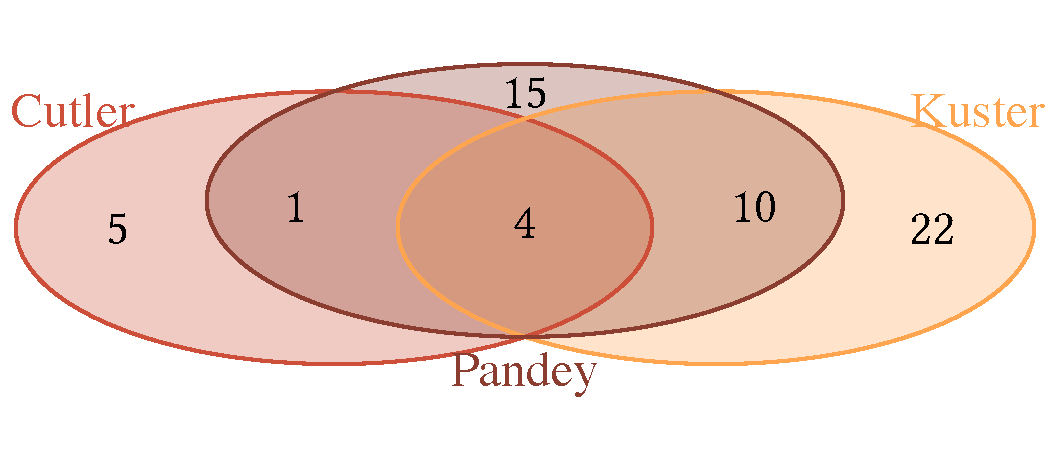
\includegraphics[scale=0.8]{proteomics/VennDiagProtCond.pdf}\centering
    \caption[Distribution of unique shared tissues between
    the 3 MS-based proteomic studies]{\label{fig:VennDiagProt3}\textbf{Distribution
    of unique and shared tissues between the 3 \ms{}-based proteomic studies.}}
\end{figure}


%\begin{figure}[!htpb]
%    \includegraphics[scale=1]{ }\centering
%    \caption[<++>]{\label{<++>}\textbf{<++>}<++>}
%\end{figure}


%\Cref{fig:VennDiagProt3}.




(1) Etat des lieux méthode 1
(2) En travaillant sur l'integration 
(3) Etat des lieux méthode 2

See \Cref{sec:ProteoData} for more details about the details of the datasets and
the pipeline.

See \Cref{subsec:distribPlot} and more particularly \Cref{fig:densityCutler_log2,%
fig:densityKuster_log2,fig:densityPandey_log2}

After exploring the transcriptomic side (way more data) I have explored the
proteomic (\ms-based) before integrating the trancriptomic to the proteomic.
It seems to be the obvious/sensible thing to do.


\section{Results}


\subsection{Disparate universe: High-throughput proteomics has a greater
variability of detection and quantification than high-throughput transcriptomics}

It is more about identification than quantification.

\subsection{About half of the quantified proteins for a given tissue are found
in different datasets}

\subsection{Technical variability seems to prevail over biological signal:
correlations between samples from a same tissue are globally lesser than
correlation between samples from a same study.}
Confirmation de la literature qui expose que la reproductibilité est compliqué


\subsection{New quantification method}

Quantification seems more rigorous than \citet{PandeyData},
but number of proteins really diminished.

Recall.
For this thesis, as it reuses available published data,
our choice for peptide assembly method is rather simple
to avoid inputting additional data that could be missing or
on which we lack enough context or perspective.
It is a variation of the optimistic model~\mycite{Huang2012-nr,Mirzaei2016-zs}.
As presented in \Cref{subsec:msDataProcess},
after selecting the peptides identified by at least two search engines
and filtered on their \gls{PSM} scores,
all the common non-null sets of peptides
(each of these sets includes its own unique peptide)
are used to assemble proteins or protein cluster
(when it is impossible to sort them out based on the list of validated peptides).
Each of these proteins or protein clusters has at least one unique peptide.
Clusters and proteins are then mapped back to \gls{Ensembl} gene identifiers.
Genes in clusters and
genes that have a protein that cover less than three unique peptides
are discarded for most of this thesis analyses.


Considered a new approach more relaxed:
while the identification is done on at least two unique peptide,
the degenerate peptides distributed across the possible proteins
similar to what cufflinks does EM algorithm.

\begin{figure}[!]
    \includegraphics[scale=0.7]{proteomics/tempo.png}\centering
    \caption[New quantification method]{\label{fig:newQuantProtMeth}\textbf{<++>}<++>}
\end{figure}

\section{Discussion}

Discuter en quoi notre méthode de ce qui a pu être écrit:
\mycite{Nesvizhskii2003-ls} peptides are apportioned among all corresponding proteins.

%%%% Maybe?
%%%Quantification with the first method
%%%Quantification with the second method with PPKM
%%%%



\section{White Board}

Less things to do than for transcriptomics.

\minisec{intro}
While \ms\ older techniques there are not tissues datasets before a couple of
years ago (2014 for Pandey, Kuster) while 2010 for Cutler.


Put the two Venn Diagrams (tissues, proteins expressed).

Cutler: older and no publication,
hard to know exactly what were the methodological protocols;but then we need to
be sure.

Super set of proteins: they are expressed in every tissues.

And then the tissues spe proteins: the one that are found in the same tissues
over the three datasets.



Conclusion Proteomics: Very hard to quantify;

Need to use Pandey (as it is the best for the analysis:
greater range of expressed proteins); pooled people (3, 2 males and one female)
and confere chapter expressed: they have better expression profile shapes.




